\documentclass[aspectratio=1610,xcolor=dvipsnames]{beamer}
\usepackage{theme}
\usepackage[utf8x]{inputenc}

\usepackage[english]{babel}
\usepackage{calligra}
\usepackage{graphicx,float,wrapfig}

\usepackage{hyperref}

\renewcommand{\bold}[1]{\textbf{\structure{#1}}}

\graphicspath{
  {../assets/}%
  }
  
\author[Conti \and Daniotti]{Samuele Conti \and Filippo Daniotti}
\title[Global Motion Estimation]{\textsc{Global Motion Estimation}}
\subtitle{A robust and hierarchical approach using an affine model}
\institute[DISI - University of Trento]{Department of Information Engineering\\and Computer Science}
\date{April 20, 2022}


\AtBeginSection[]
{
    \begin{frame}
        \frametitle{Table of Contents}
        \tableofcontents[currentsection]
    \end{frame}
}

\begin{document}

\begin{frame}
    \titlepage
    \begin{figure}[H]
        \begin{center}
            
\includegraphics[width=0.4\linewidth]{marchio_unitrento_colore_it_202002.eps}
        \end{center}
    \end{figure}
\end{frame}

\begin{frame}
    \tableofcontents[sectionstyle=show,subsectionstyle=show/shaded/hide,subsubsectionstyle=show/shaded/hide]
\end{frame}

\section{Introduction}
\begin{frame}{Introduction}
    In this work we are going to present:
    \begin{itemize}
        \item a broad introduction to the problem of global motion estimation
        \item an overview of the wide body of literature that covers the problem
        \item the framework we developed from the aforementioned literature
        \item an analysis of the performances of our solution
        \item a brief discussion of the limitations and possible improvements of our solution
    \end{itemize}
\end{frame}

\section{The problem}
\begin{frame}{Motion estimation}
    The problem of motion estimation aims to produce an estimate of the movement of the objects in a video
    \bigskip
    \begin{itemize}
        \item idea: the difference between two frames gives information on the motion in the scene
        \item ideally, we could be able to estimate the direction and velocity of any object of interest
        \item camera movements pollute such estimate
        \begin{itemize}
            \item they introduce apparent motion for every object
        \end{itemize} 
    \end{itemize}
\end{frame}

\begin{frame}{Global motion stimation}
    Global motion estimation aims to compute an estimate of the global motion field patterns introduced by the camera
    \bigskip
    \begin{itemize}
        \item idea: subtract the global motion from the motion field
        \begin{itemize}
            \item this should highlight the local motion of the objects
        \end{itemize} 
        \item removing camera motion is useful in a virety of applications:
        \begin{itemize}
            \item when dealing unwanted motion from a video 
            \item when we are interested in the ego-motion
        \end{itemize}
    \end{itemize}    
\end{frame}

\section{Literature}
\begin{frame}{Dealing with GME}
    Most of the existing algorithms that deal with global motion estimation assume that camera motion can be described as a  \bold{parameterized motion model}.
    \begin{block}{Parameterized motion model}
        It is an equation that describes the expected shape of the motion vector for each still pixel, given a certain movement of the camera
    \end{block}
    \bigskip
    Different models describe different types of motion (translation, rotation, panning, et cetera)
    \begin{exampleblock}{Well-established models}
        \begin{itemize}
            \item translation model
            \item affine model (our choice)
            \item projective model
        \end{itemize}
    \end{exampleblock}
\end{frame}

\begin{frame}{Estimating parameters}
    Once the choice of the motion model has been made, there are two main approaches for estimating the parameters
    \bigskip
    \begin{itemize}
        \item direct methods
        \item indirect methods
    \end{itemize}
    \bigskip
    For our solution we went for \bold{indirect} methods
\end{frame}

\section{Implementation}
\begin{frame}{Overview}
    Three are the main operations that constitute the framework that we have developed:
    \bigskip
    \begin{enumerate}
        \item \bold{motion estimation}: compute a dense motion field for a given frame
        \item \bold{global motion estimation}: compute the motion model parameters
        \item \bold{motion compensation}: subtract GME from the dense motion field to get a compensated frame
    \end{enumerate}
\end{frame}

\subsection{Dense motion estimation}
\begin{frame}{Block-based motion estimation}
	The affine model requires a dense motion field when computing the parameters, which can be computed using a block-based approach

	\bigskip	
	We implemented 4 well-established BBME algorithms:
	\begin{itemize}
		\item exhaustive search
		\item three-step search
		\item 2D log search
		\item diamond search
	\end{itemize}
	\bigskip
	As DFD, we tried both 1-norm and 2-norm
    
\end{frame}

\begin{frame}{Exhaustice search}
	\begin{columns}
		\begin{column}{0.5\textwidth}
			\begin{figure}
				\centering
				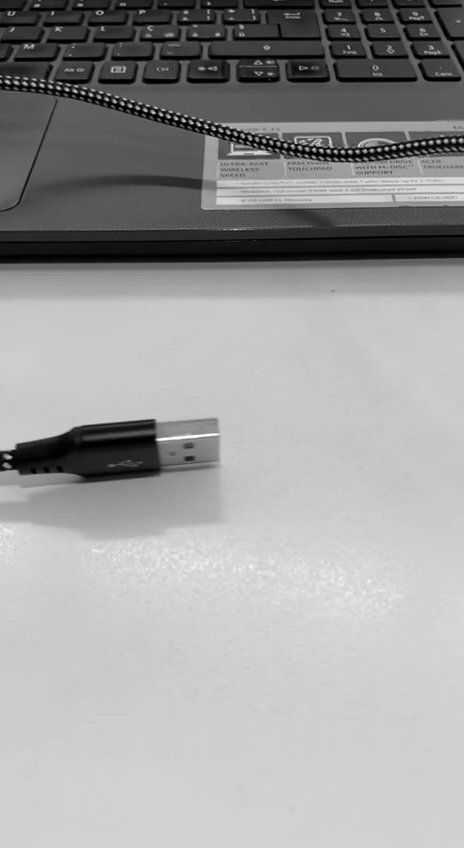
\includegraphics[keepaspectratio, width=.5\linewidth]{images/bbme-im.png}
			\end{figure}
		\end{column}
		\begin{column}{0.5\textwidth}
			\begin{figure}
				\centering
				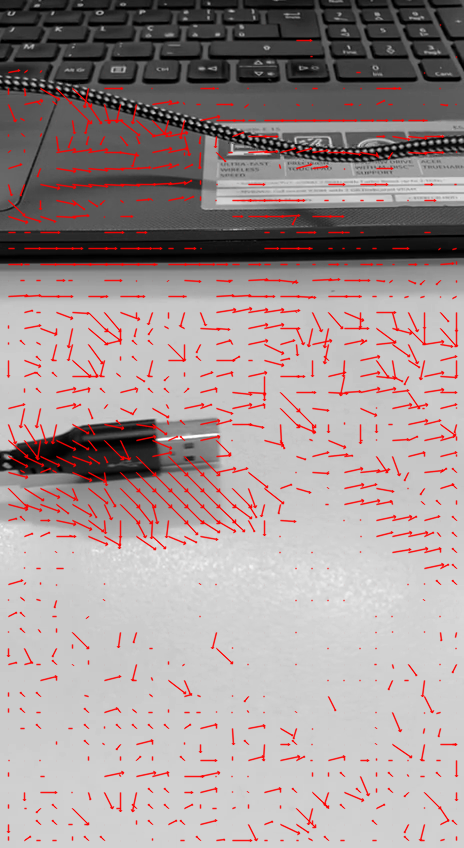
\includegraphics[keepaspectratio, width=.5\linewidth]{images/bbme-0-res.png}
			\end{figure}
		\end{column}
	\end{columns}
\end{frame}

\begin{frame}{Three-step search}
	
	\begin{columns}
		\begin{column}{0.5\textwidth}
			\begin{figure}
				\centering
				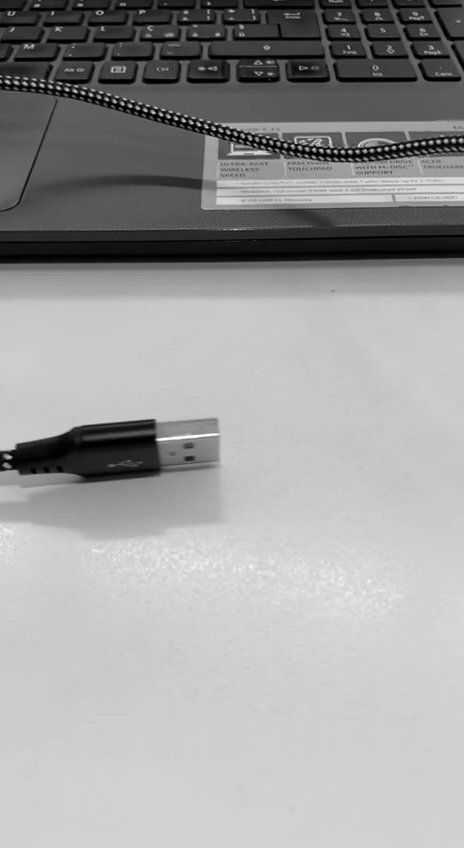
\includegraphics[keepaspectratio, width=.5\linewidth]{images/bbme-im.png}
			\end{figure}
		\end{column}
		\begin{column}{0.5\textwidth}
			\begin{figure}
				\centering
				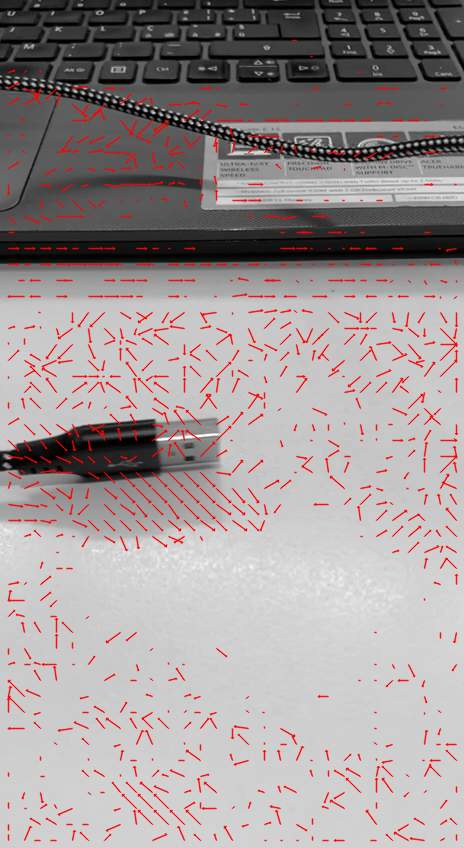
\includegraphics[keepaspectratio, width=.5\linewidth]{images/bbme-1-res.png}
			\end{figure}
		\end{column}
	\end{columns}
\end{frame}

\begin{frame}{2D Log search}
	
	\begin{columns}
		\begin{column}{0.5\textwidth}
			\begin{figure}
				\centering
				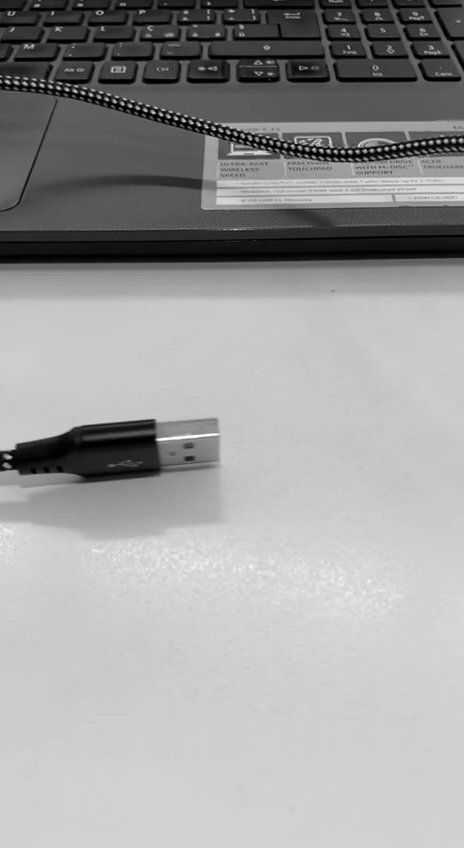
\includegraphics[keepaspectratio, width=.5\linewidth]{images/bbme-im.png}
			\end{figure}
		\end{column}
		\begin{column}{0.5\textwidth}
			\begin{figure}
				\centering
				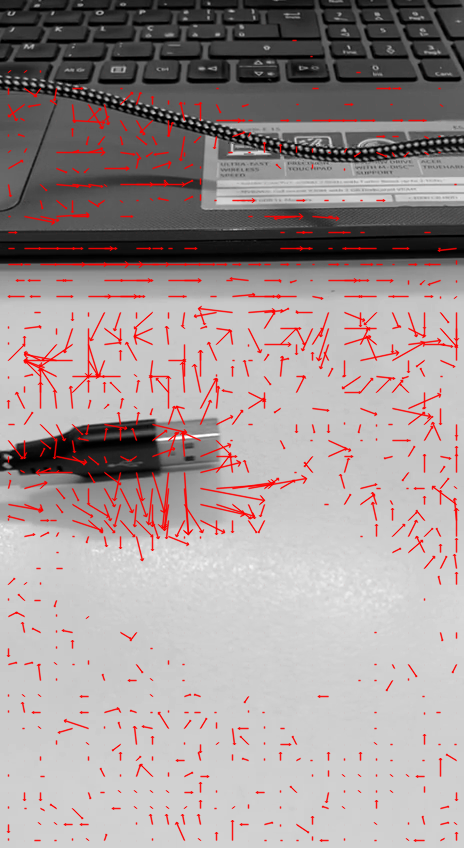
\includegraphics[keepaspectratio, width=.5\linewidth]{images/bbme-2-res.png}
			\end{figure}
		\end{column}
	\end{columns}
\end{frame}

\begin{frame}{Diamond search}
	
	\begin{columns}
		\begin{column}{0.5\textwidth}
			\begin{figure}
				\centering
				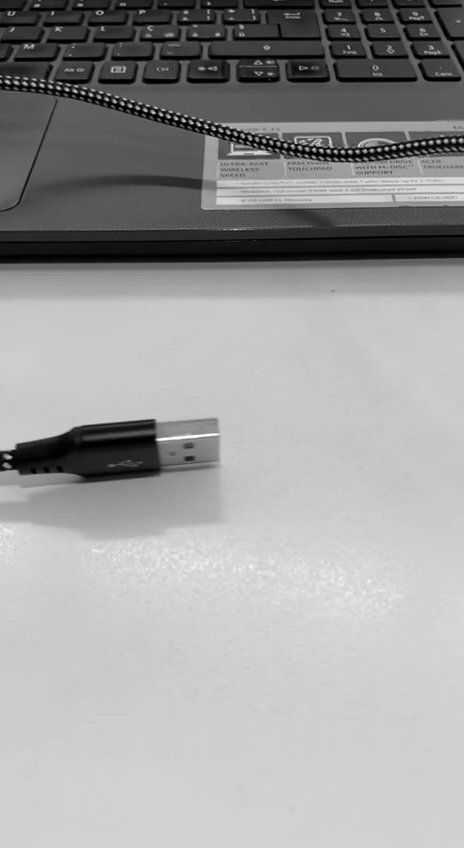
\includegraphics[keepaspectratio, width=.5\linewidth]{images/bbme-im.png}
			\end{figure}
		\end{column}
		\begin{column}{0.5\textwidth}
			\begin{figure}
				\centering
				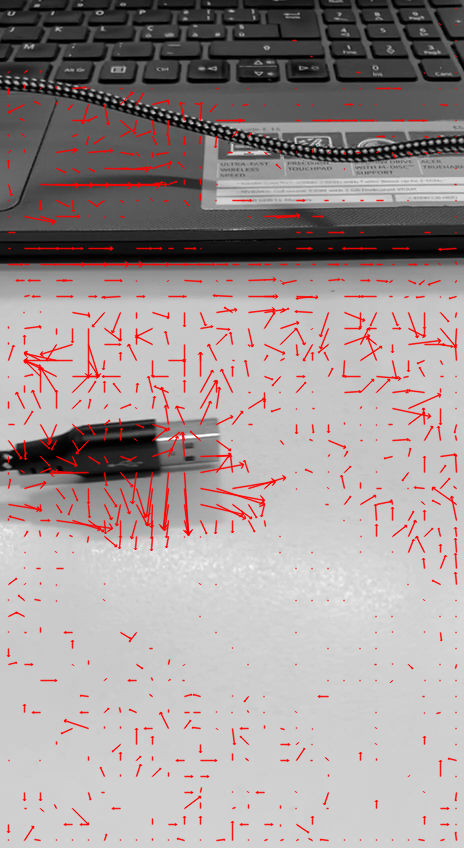
\includegraphics[keepaspectratio, width=.5\linewidth]{images/bbme-3-res.png}
			\end{figure}
		\end{column}
	\end{columns}
\end{frame}

\subsection{The affine model}
\begin{frame}{Affine model}
    
\end{frame}

\subsection{Refinement: robust and hierarchical GME}
\subsection{Motion compensation}
\begin{frame}{Compensation}
    
\end{frame}

\section{Performances}

\section{Conclusions}

\begin{frame}
    \begin{center}
        {\Huge\calligra Thanks!}
    \end{center}
\end{frame}

\end{document}